\documentclass[11pt]{article}

\usepackage{amsmath}
\usepackage{float}
\usepackage{graphicx}
\usepackage{subcaption}

\begin{document}

    \title{HPCSE II - Exercise 2}
    \author{Anian Ruoss}
    \maketitle

    \subsection*{Task 4}
    \label{subsec:Task4}

    \begin{figure}[H]
        \begin{center}
            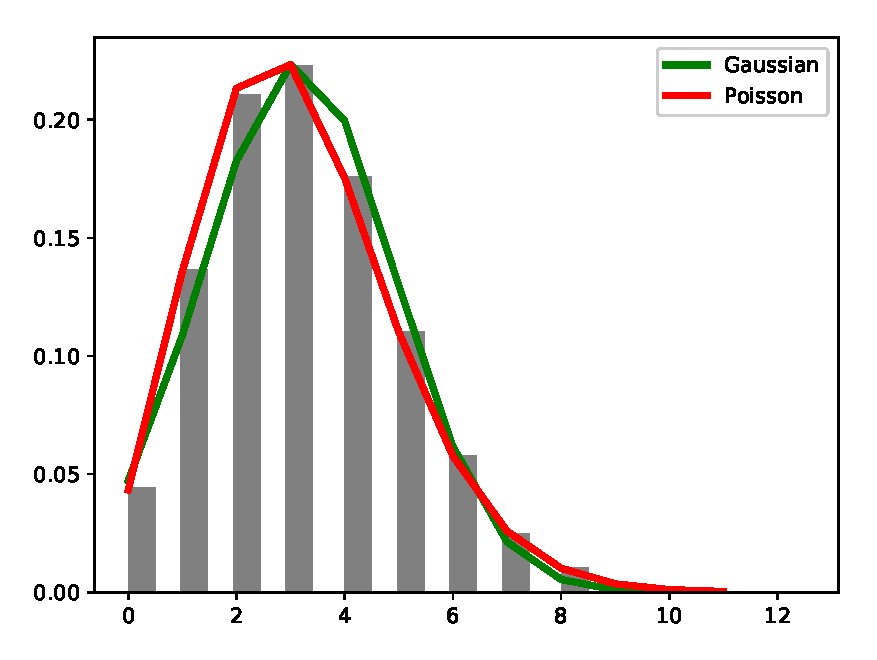
\includegraphics[width=.75\textwidth]{plots/hist_distributions.eps}
        \end{center}
        \caption{Normalized histogram with 100 bins and distributions from MLE
        parameters
        $\left(
        \hat{\lambda}_{\text{MLE}} = \hat{\mu}_{\text{MLE}} \approx 3.14
        \text{ and } \hat{\sigma}_{\text{MLE}} \approx 3.17 \right)$.
        The Poisson distribution clearly provides a better fit than the
        Gaussian.
        This agrees with the fact that maximum log-likelihood for the
        Poisson distribution is larger than the Gaussian's.
        As hypothesized, the data does not reflect the symmetry imposed by a
        Gaussian distribution.}
    \end{figure}

    \subsection*{Task 5}
    \label{subsec:Task5}

    \begin{figure}[H]
        \begin{center}
            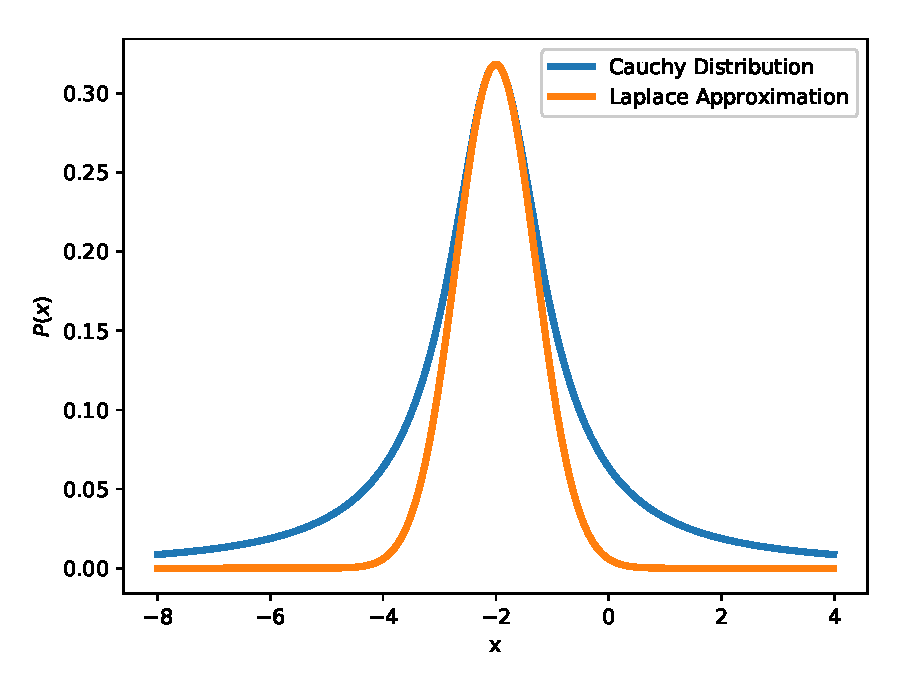
\includegraphics[width=.75\textwidth]{plots/laplace_approximation.eps}
        \end{center}
        \caption{Cauchy distribution for $x_{0} = -2 \text{ and } \gamma = 1$
        and the corresponding Laplace approximation around $\hat{x} = x_{0}$.}
    \end{figure}

\end{document}
